% % % \begin{appendix}
% % % \section{Messdaten}
% % % \centering
% % % \begin{figure}
% % % \includepdf[width=0.9\textwidth, pages={1}]{Bilder/Messdaten.pdf}
% % % \end{figure}
% % % \newpage
% % % \begin{figure}
% % % \includepdf[width=0.9\textwidth, pages={2}]{Bilder/Messdaten.pdf}
% % % \end{figure}
% % %
% % % \end{appendix},


% % % % Standard Plot
% \begin{figure}
%   \centering
%   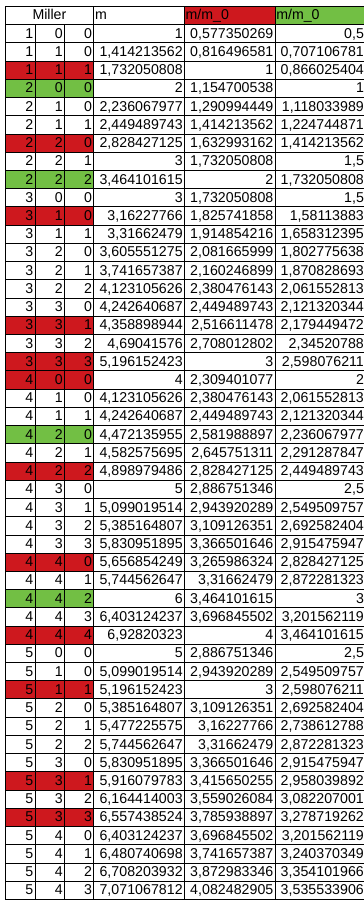
\includegraphics{ressources/Steinsalz.png}
%   \caption{Millerindizes und das theoretische Verhältnis nach \ref{eq:dm} für die Steinsalz/Fluorit-Struktur (a). Die grün hinterlegten Felder stellen schwache und die rot hinterlegten Felder starke Reflexe dar.}
%   \label{fig:Anhang1}
% \end{figure}

% \begin{figure}
%   \centering
%   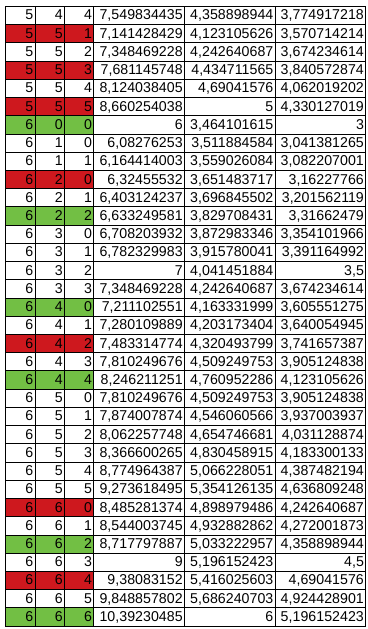
\includegraphics{ressources/Steinsalz2.png}
%   \caption{Millerindizes für die Steinsalz/Fluorit-Struktur (b).}
%   \label{fig:Anhang2}
% \end{figure}

% \begin{figure}
%   \centering
%   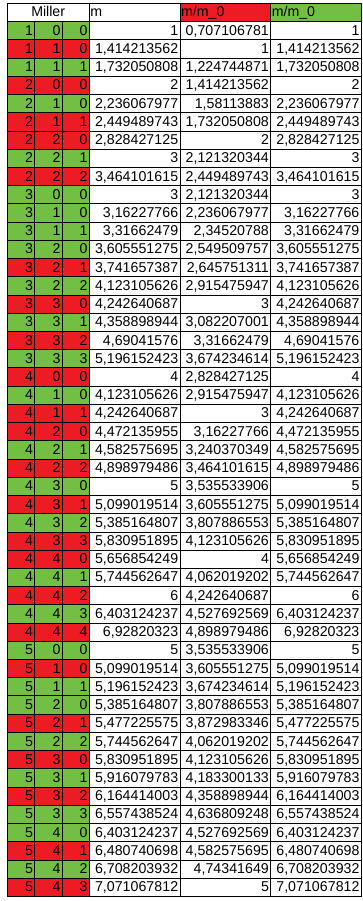
\includegraphics{ressources/Caesium.png}
%   \caption{Millerindizes und das theoretische Verhältnis nach \ref{eq:dm} für die Caesium-Struktur (a). Die grün hinterlegten Felder stellen schwache und die rot hinterlegten Felder starke Reflexe dar.}
%   \label{fig:Anhang3}
% \end{figure}

% \begin{figure}
%   \centering
%   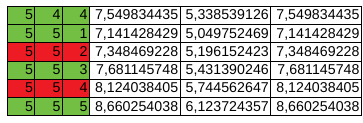
\includegraphics{ressources/Caesium2.png}
%   \caption{Millerindizes für die Caesium-Struktur (b).}
%   \label{fig:Anhang4}
% \end{figure}

% \begin{figure}
%   \centering
%   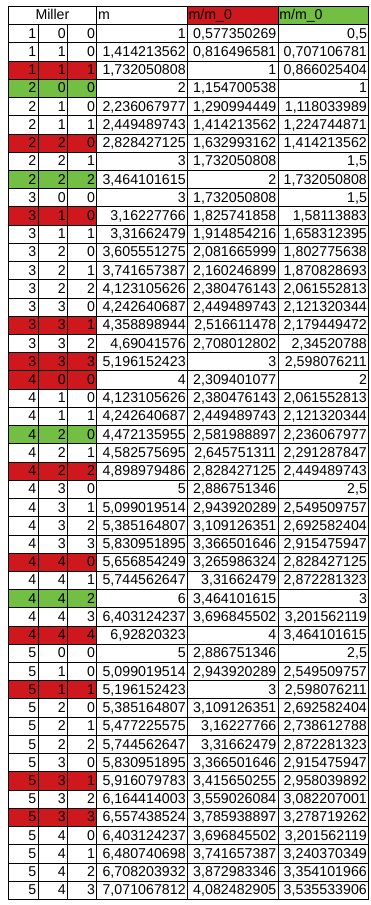
\includegraphics{ressources/Zinkblende.png}
%   \caption{Millerindizes und das theoretische Verhältnis nach \ref{eq:dm} für die Zinkblende-Struktur (a). Die grün hinterlegten Felder stellen schwache und die rot hinterlegten Felder starke Reflexe dar.}
%   \label{fig:Anhang5}
% \end{figure}

% \begin{figure}
%   \centering
%   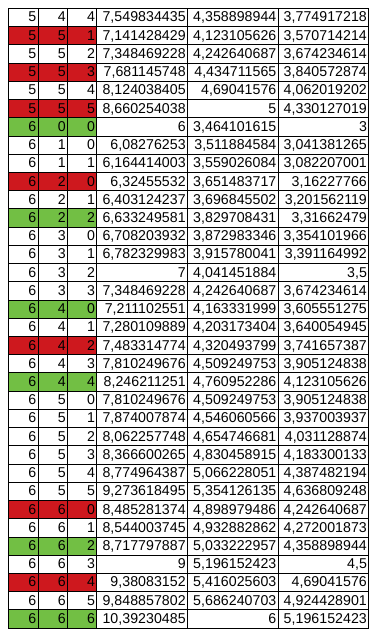
\includegraphics{ressources/Zinkblende2.png}
%   \caption{Millerindizes für die Zinblenden-Struktur (b).}
%   \label{fig:Anhang6}
% \end{figure}